\documentclass{article}

\usepackage{graphicx}
\usepackage{subfig}
\usepackage{multirow}
\title{{\bf Supplementary Material:} \\A causal web between chronotype and metabolic health traits}
https://www.overleaf.com/project/605b6416422edc98436c7254
\author{}
\date{}

\begin{document}
\maketitle

% omega 3 and total triglycerides
\begin{figure}[htbp]
     \centering
     \begin{subfigure}[b]{0.4\textwidth}
         \centering
         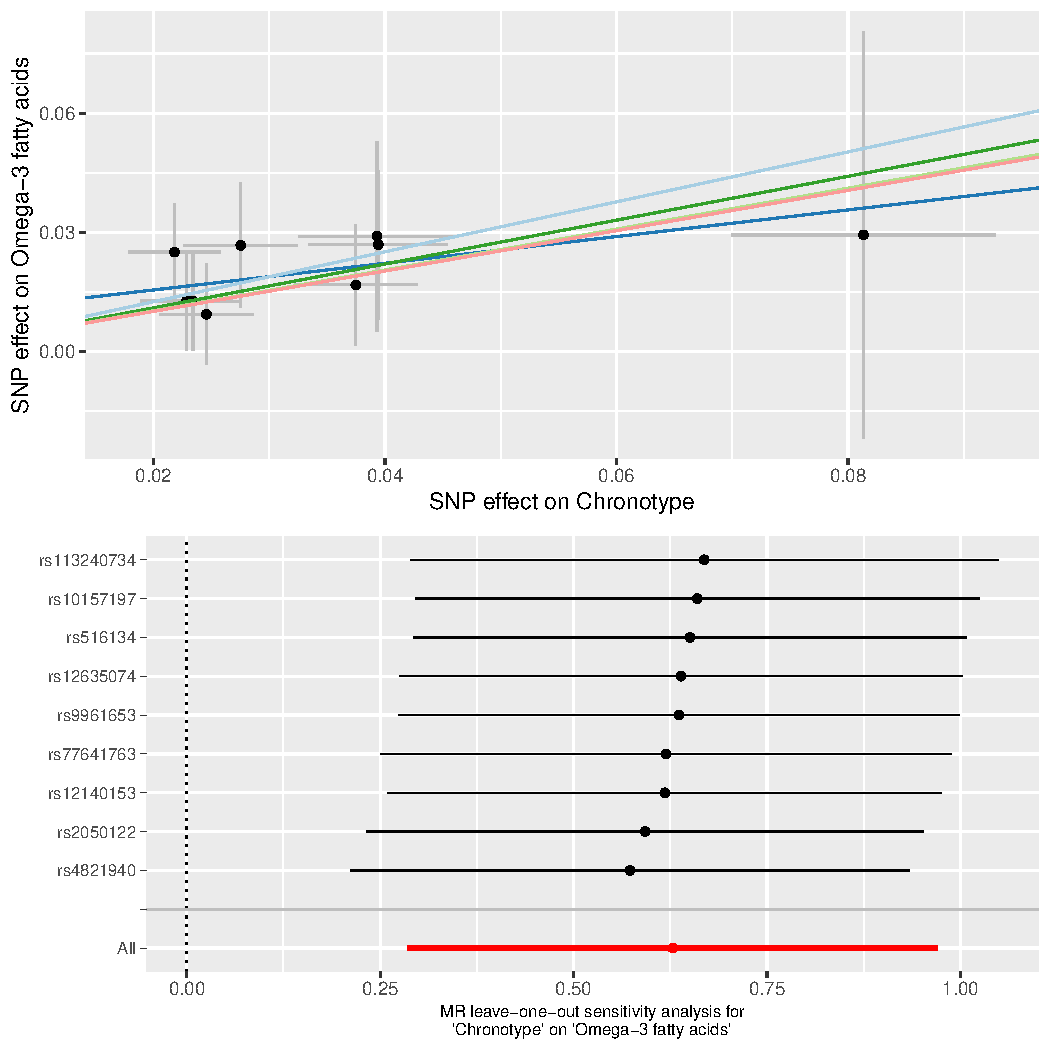
\includegraphics[width=0.4\textwidth]{Figs/Analysis2/Chronotype_vs_Omega-3_fatty_acids.Plots.pdf}
         %\caption{}
         \label{omega3}
     \end{subfigure}
     \begin{subfigure}[b]{0.4\textwidth}
         \centering
         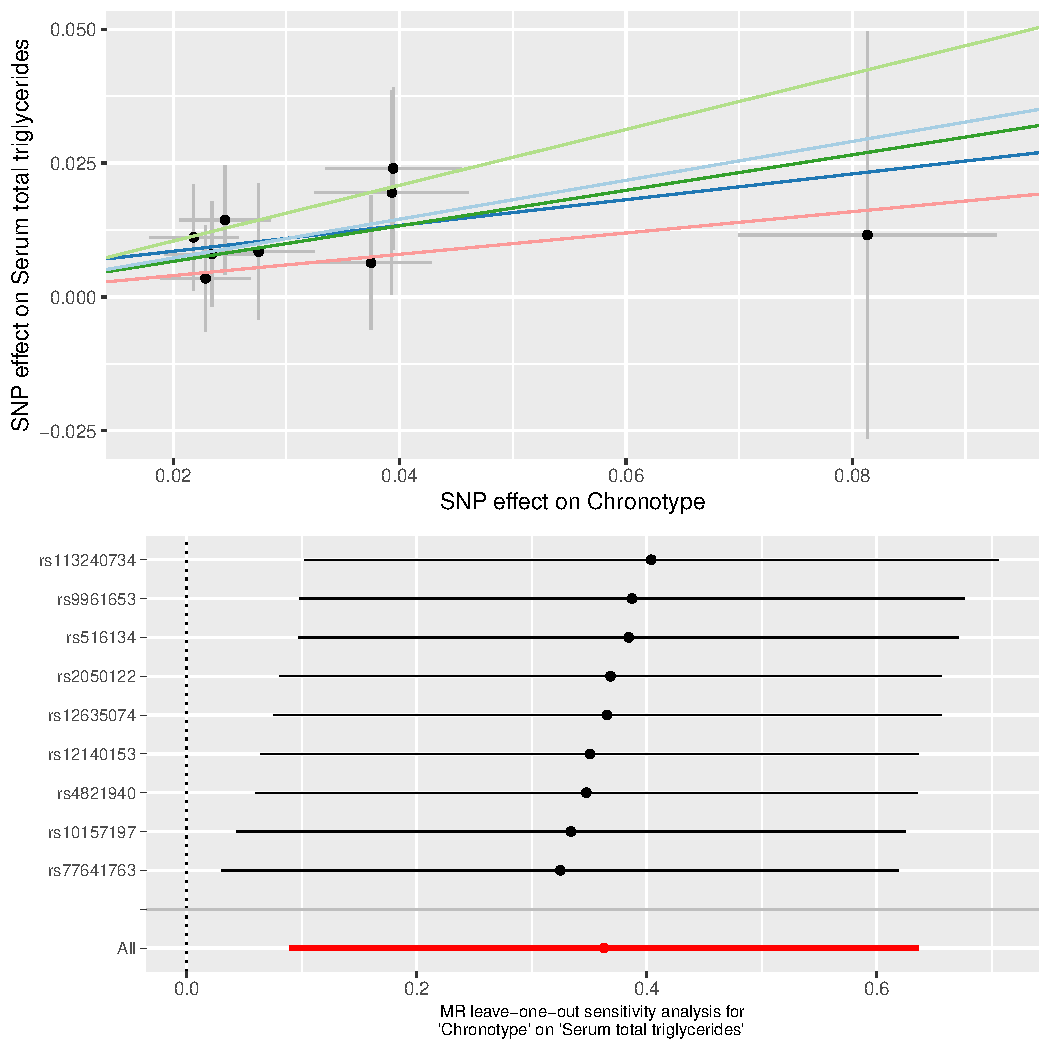
\includegraphics[width=0.4\textwidth]{Figs/Analysis2/Chronotype_vs_Serum_total_triglycerides.Plots.pdf}
         %\caption{}
         \label{totalTG}
     \end{subfigure}
        \caption{Propensity to an evening chronotype causes increased omega-3 fatty acids (A) and serum total triglycerides (B). IVW, Weighted median, mode, weighted mode, and Egger regressions shown. Lower panels depict leave-one-out sensitivity analyses with the IVW method.}
        \label{omega3tgs}
\end{figure}

% total ffa and nicorandil
\begin{figure}[htbp]
     \centering
     \begin{subfigure}[b]{0.4\textwidth}
         \centering
         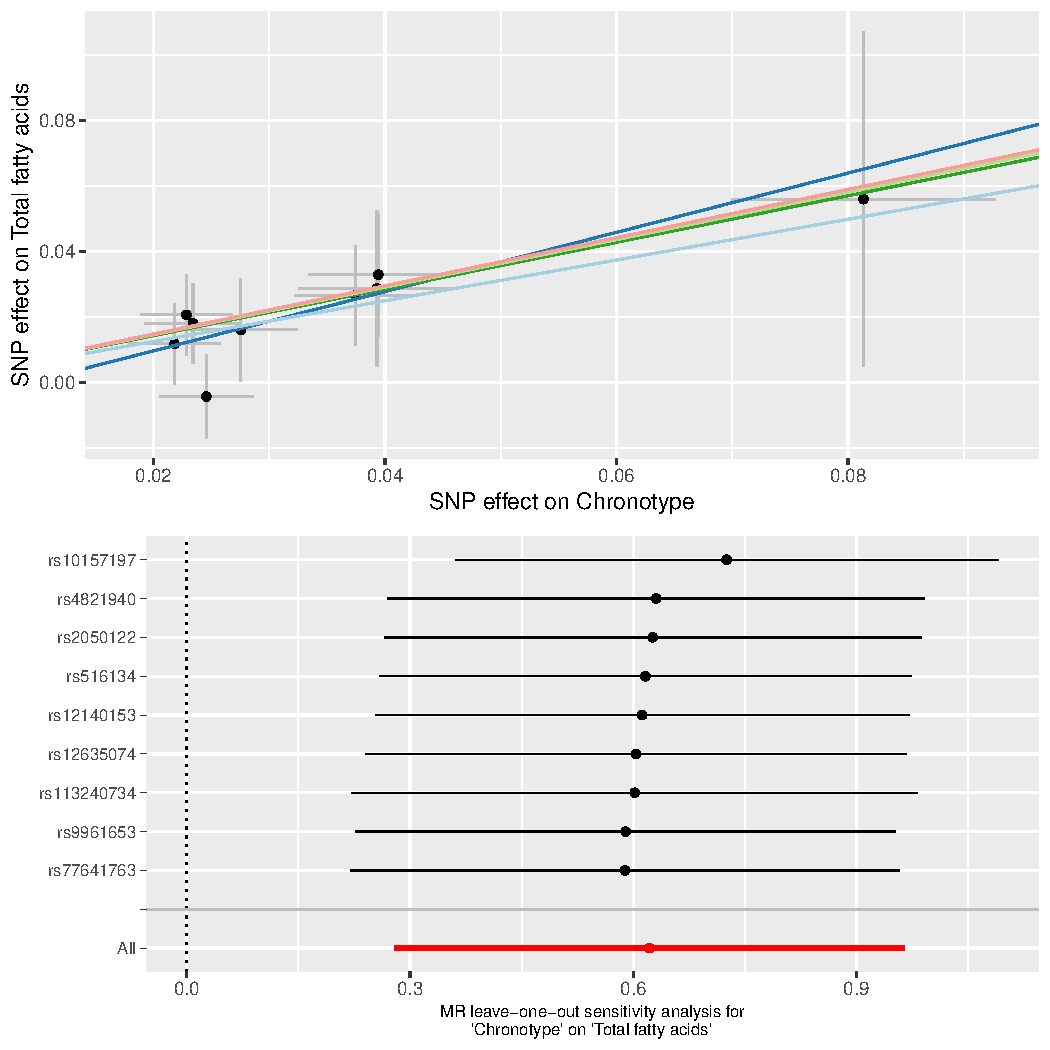
\includegraphics[width=\textwidth]{Figs/Analysis2/Chronotype_vs_Total_fatty_acids.Plots.pdf}
         \caption{}
         \label{tffa}
     \end{subfigure}
     \begin{subfigure}[b]{0.4\textwidth}
         \centering
         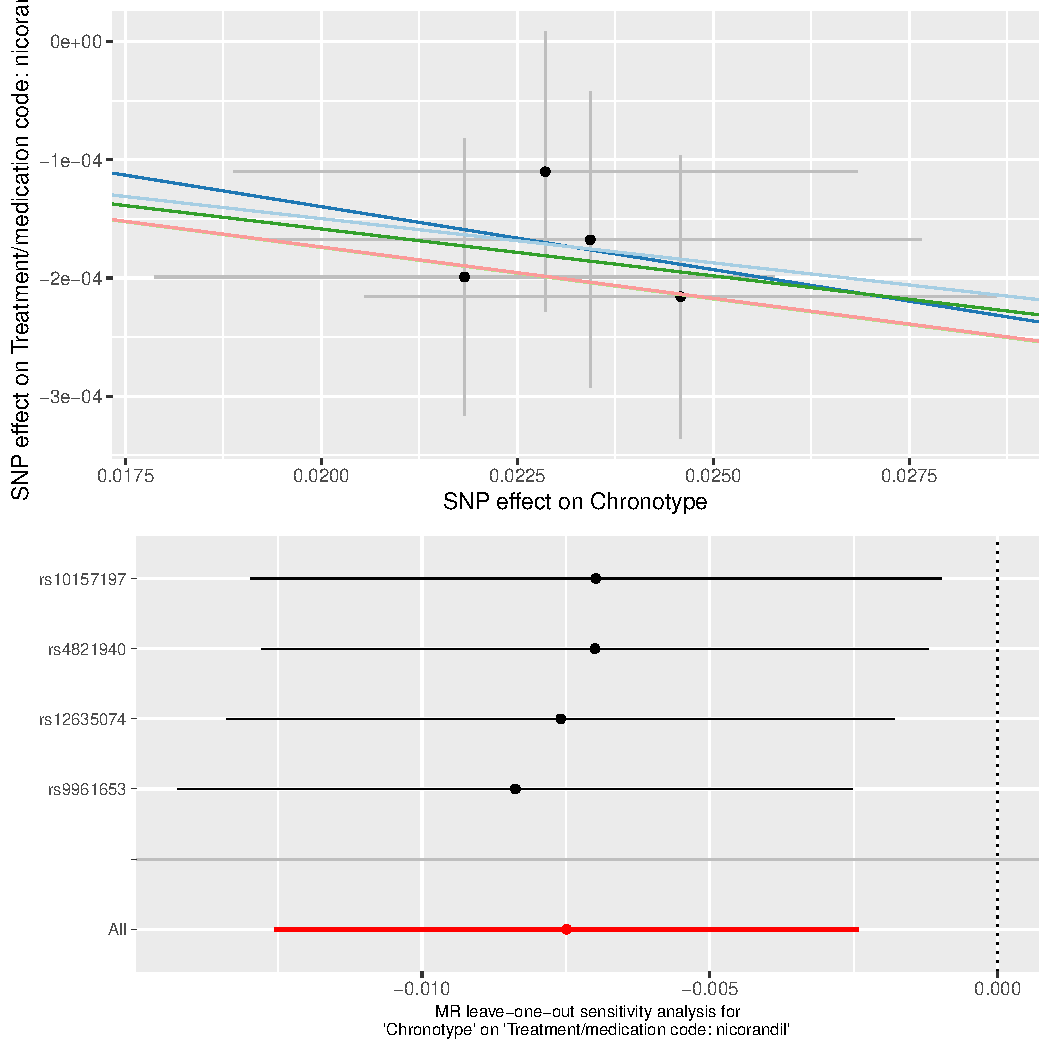
\includegraphics[width=\textwidth]{Figs/Analysis2/Chronotype_vs_Treatment_medication_code:_nicorandil.Plots.pdf}
         \caption{}
         \label{nicorandil}
     \end{subfigure}
        \caption{Chronotype causes increased total fatty acids (A) and and a decreased likelihood of treatment with nicorandil. IVW, Weighted median, mode, weighted mode, and Egger regressions shown. Lower panels depict leave-one-out sensitivity analyses with the IVW method.}
        \label{fffanicorandil}
\end{figure}


% total T2dm and alcohol
\begin{figure}[htbp]
     \centering
     \begin{subfigure}[b]{0.4\textwidth}
         \centering
         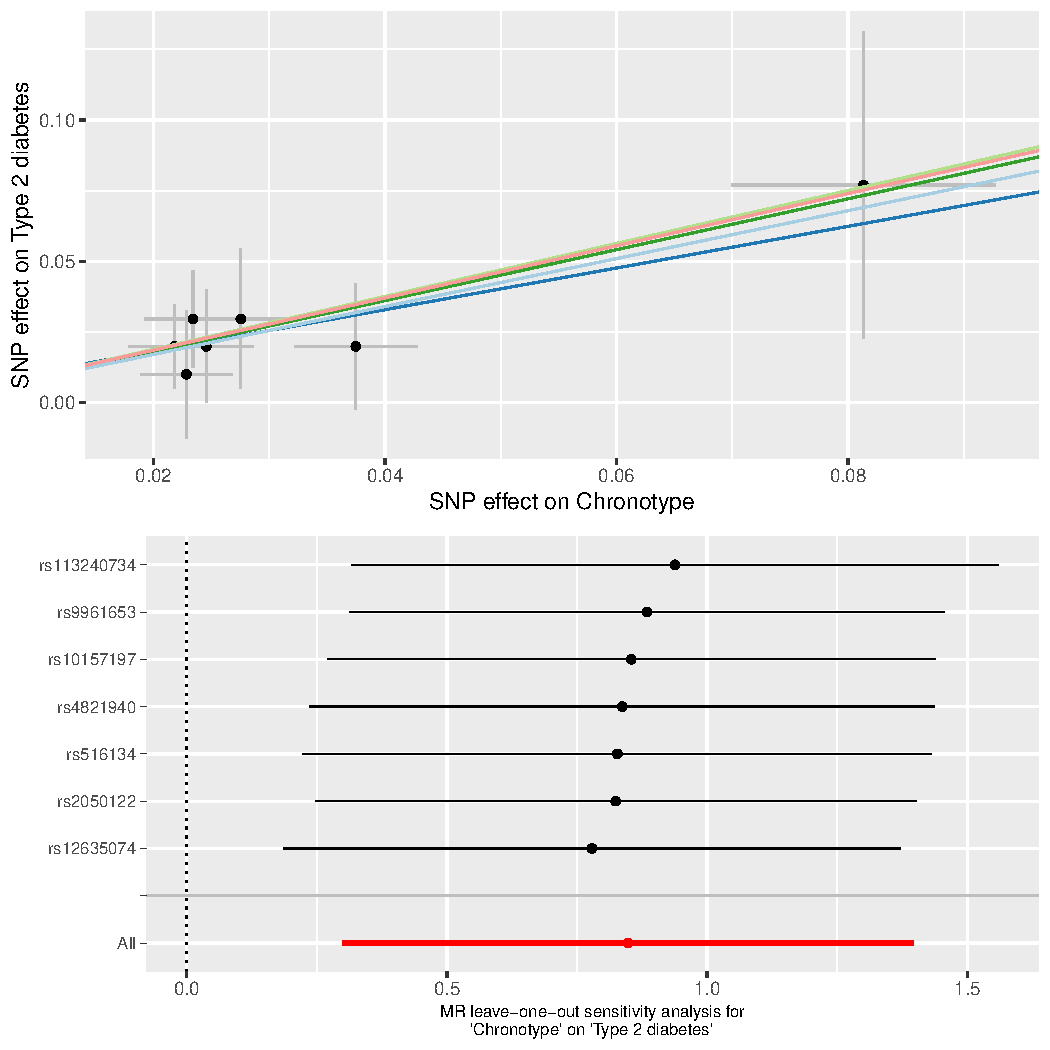
\includegraphics[width=\textwidth]{Figs/Analysis2/Chronotype_vs_Type_2_diabetes.Plots.pdf}
         \caption{}
         \label{t2dm}
     \end{subfigure}
     \begin{subfigure}[b]{0.4\textwidth}
         \centering
         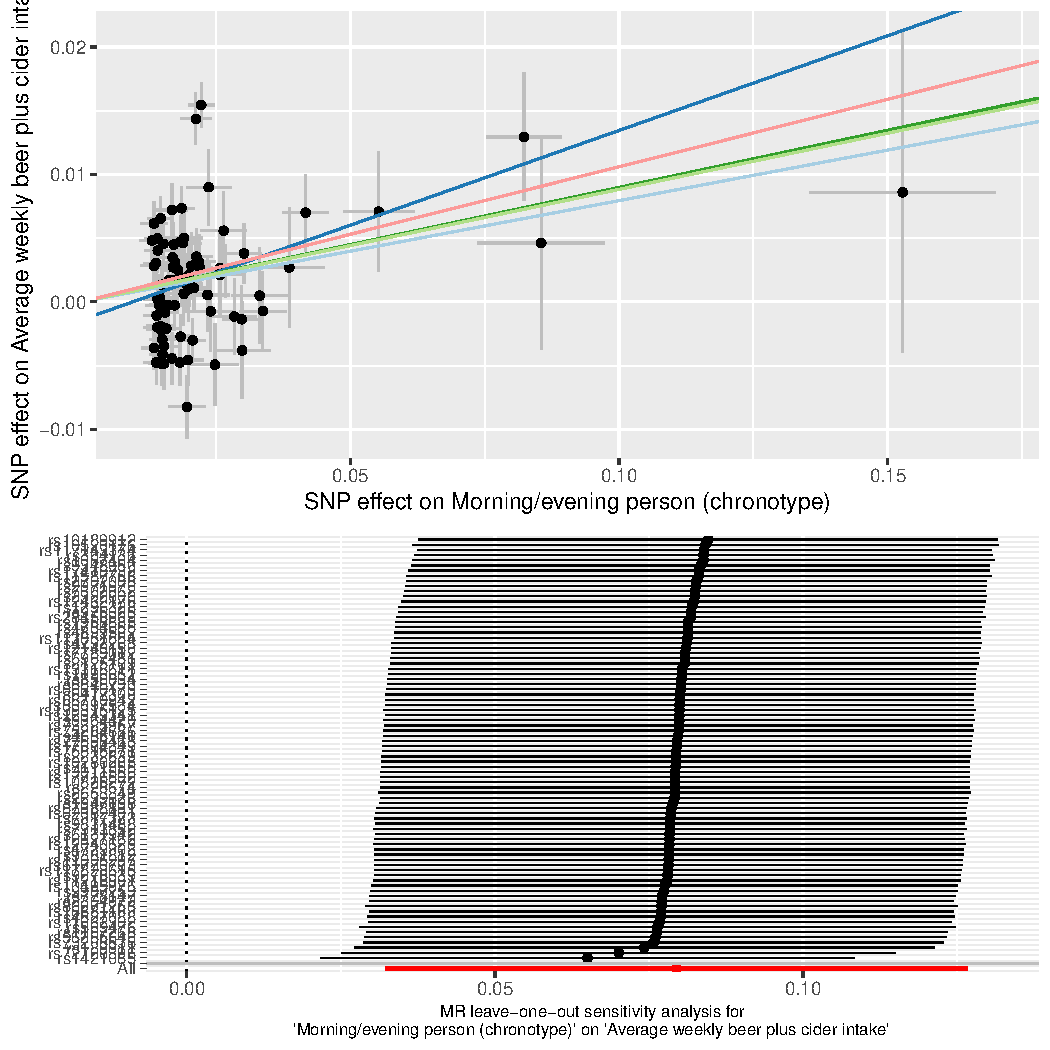
\includegraphics[width=\textwidth]{Figs/Analysis2/Morning_evening_person_(chronotype)_vs_Average_weekly_beer_plus_cider_intake.Plots.pdf}
         \caption{}
         \label{beer}
     \end{subfigure}
        \caption{Chronotype causes increased odds of a type 2 diabetes mellitus diagnosis (A) and and an increased weekly beer/cider intake. IVW, Weighted median, mode, weighted mode, and Egger regressions shown. Lower panels depict leave-one-out sensitivity analyses with the IVW method.}
        \label{t2dmalcohol}
\end{figure}

% total bp and tired
\begin{figure}[htbp]
     \centering
     \begin{subfigure}[b]{0.4\textwidth}
         \centering
         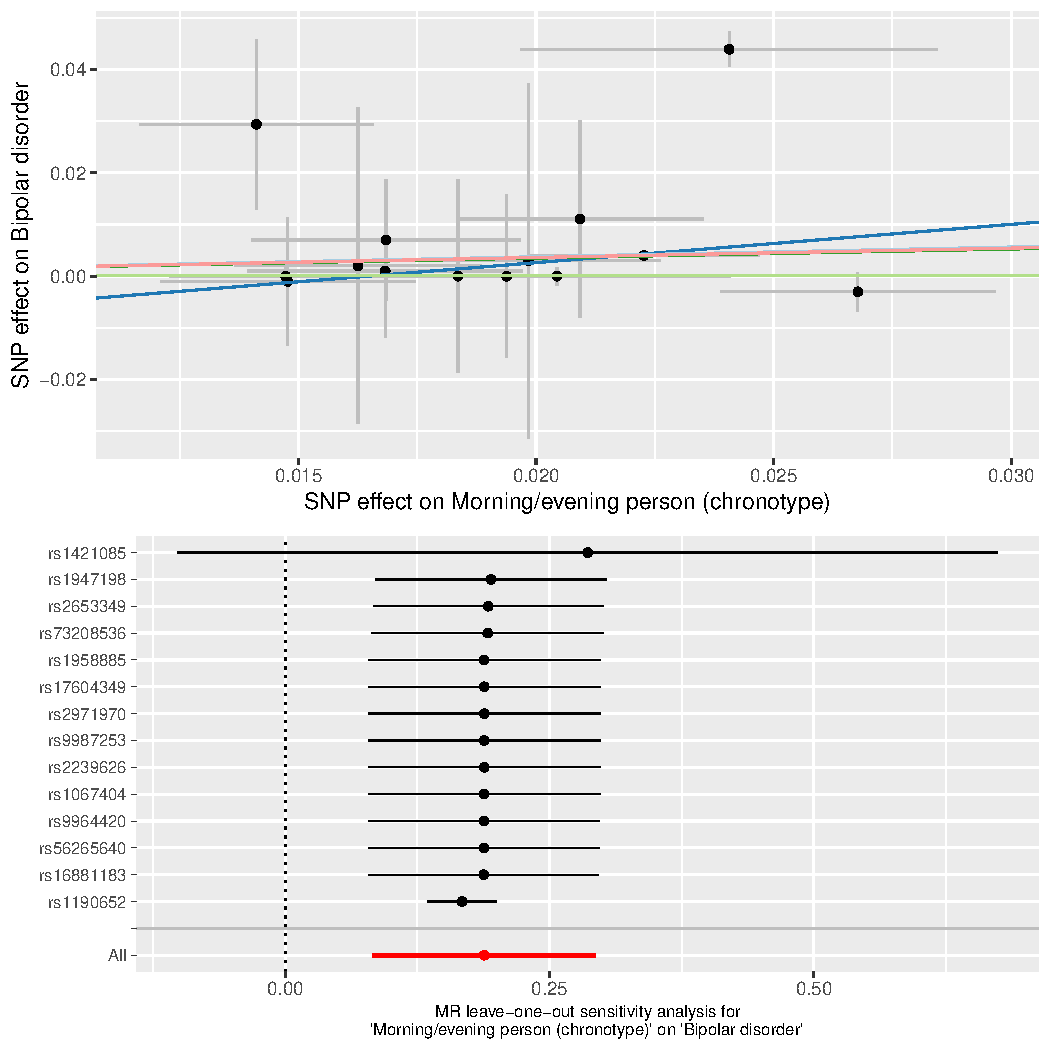
\includegraphics[width=\textwidth]{Figs/Analysis2/Morning_evening_person_(chronotype)_vs_Bipolar_disorder.Plots.pdf}
         \caption{}
         \label{t2dm}
     \end{subfigure}
     \begin{subfigure}[b]{0.4\textwidth}
         \centering
         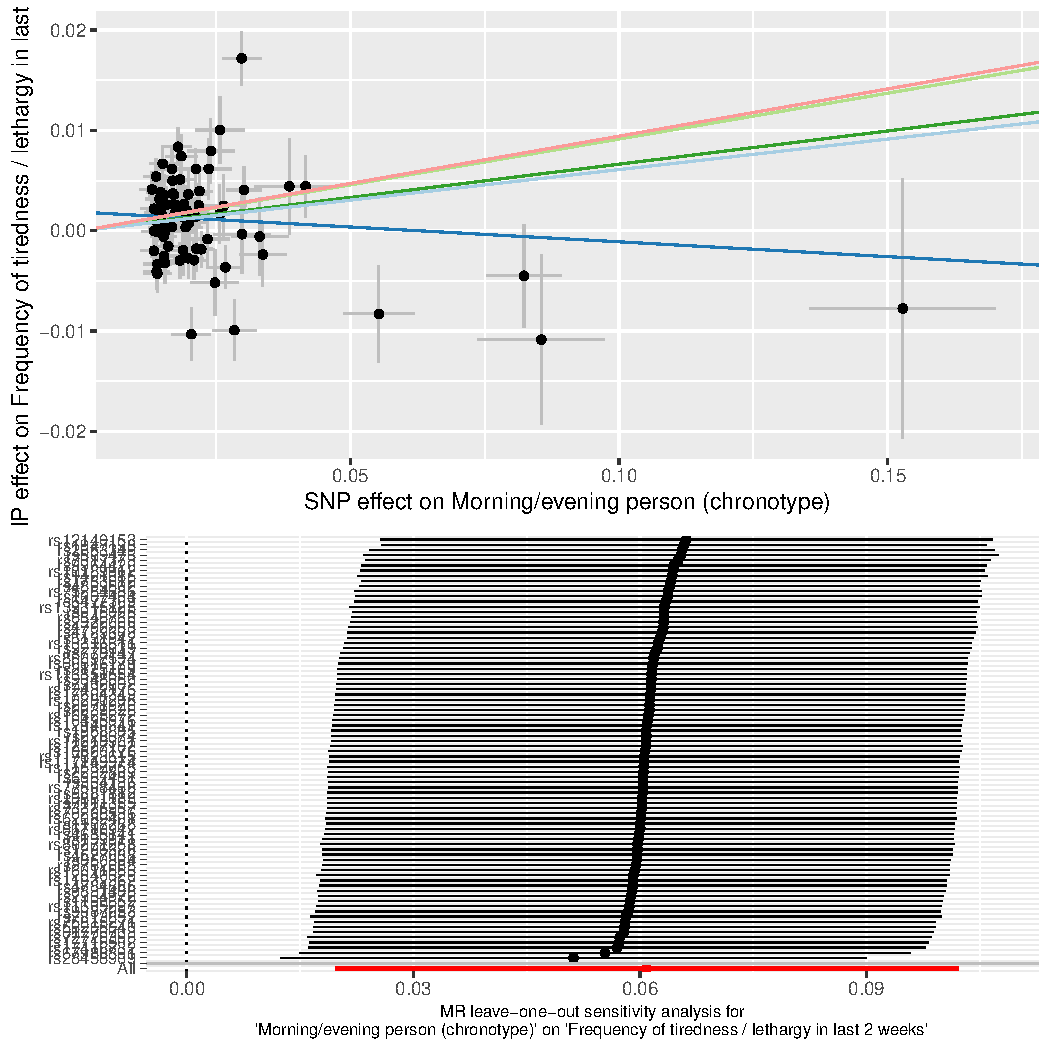
\includegraphics[width=\textwidth]{Figs/Analysis2/Morning_evening_person_(chronotype)_vs_Frequency_of_tiredness___lethargy_in_last_2_weeks.Plots.pdf}
         \caption{}
         \label{beer}
     \end{subfigure}
        \caption{An evening chronotype contributes to a bipolar disorder diagnosis (A) and self-reported lethargy. IVW, Weighted median, mode, weighted mode, and Egger regressions shown. Lower panels depict leave-one-out sensitivity analyses with the IVW method.}
        \label{bplethargy}
\end{figure}

% total test and wakingearly
\begin{figure}[htbp]
     \centering
     \begin{subfigure}[b]{0.4\textwidth}
         \centering
         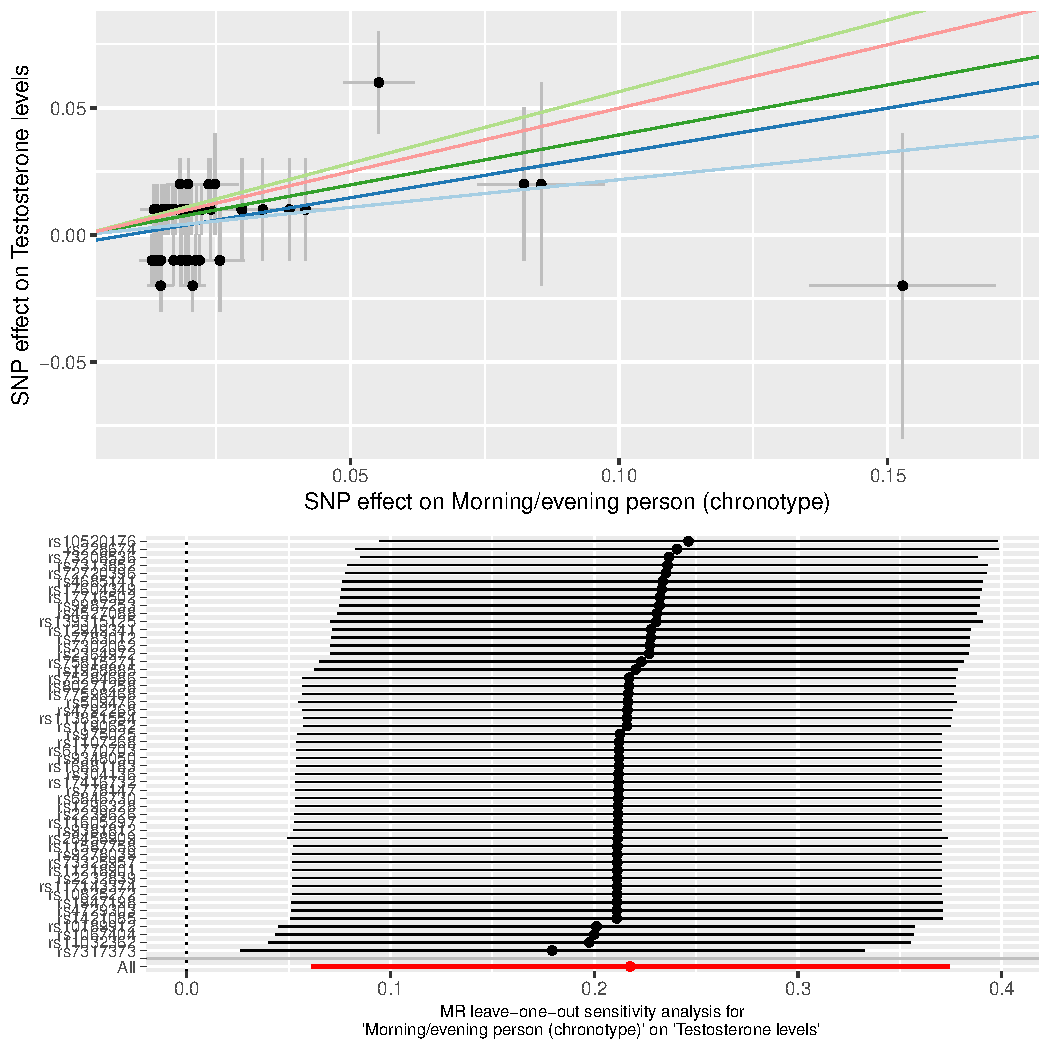
\includegraphics[width=\textwidth]{Figs/Analysis2/Morning_evening_person_(chronotype)_vs_Testosterone_levels.Plots.pdf}
         \caption{}
         \label{testosterone}
     \end{subfigure}
     \begin{subfigure}[b]{0.4\textwidth}
         \centering
         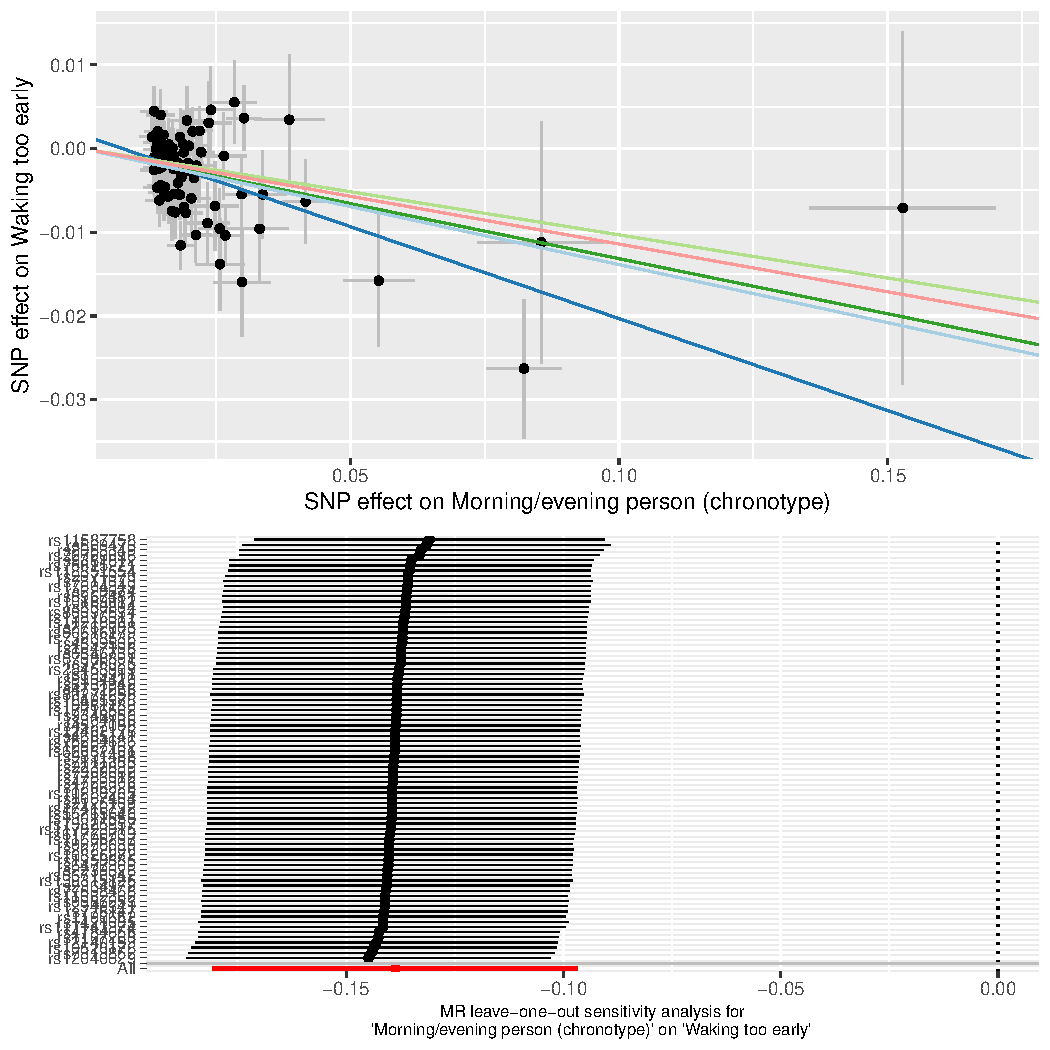
\includegraphics[width=\textwidth]{Figs/Analysis2/Morning_evening_person_(chronotype)_vs_Waking_too_early.Plots.pdf}
         \caption{}
         \label{waking}
     \end{subfigure}
        \caption{An evening chronotype contributes to increased serum testosterone (A) and a decrease in odds of waking early. IVW, Weighted median, mode, weighted mode, and Egger regressions shown. Lower panels depict leave-one-out sensitivity analyses with the IVW method.}
        \label{t2dmalcohol}
\end{figure}







% \renewcommand{\arraystretch}{1.5}
% \setlength{\tabcolsep}{4pt}
% \begin{table*}[ht!]
% \resizebox{\textwidth}{!}{
% \begin{tabular}{lll}
% \hline
% {\bf Index} & Unipartite Graph& Bipartite graph\\
% \hline
% CN & $Z_{uv}^{CN} = \left|\{\Gamma(x) \cap \Gamma(y)\} \right|$ & $S_{uv}^{CN} = \left|\{\widehat{\Gamma}(x) \cap \Gamma(y)\} \cup \{\Gamma(x) \cap \widehat{\Gamma}(y)\}\right|$\\
% JC & $Z_{uv}^{JC} = \frac{Z_{uv}^{CN}} {\left|\Gamma(x) \cup \Gamma(y)\right|}$ & $S_{uv}^{JC} = \frac{S_{uv}^{CN}} {\left|\Gamma(x) \cup \Gamma(y)\right|}$ \\
% AA & $Z_{uv}^{AA} = \sum_{z\in \{\{\widehat{\Gamma}(x) \cap \Gamma(y)\} \cup \{\Gamma(x) \cap \widehat{\Gamma}(y)\}\}} \frac{1}{\log_2\left|\Gamma(z)\right|}$ & $S_{uv}^{AA} = \sum_{z\in \{\{\widehat{\Gamma}(x) \cap \Gamma(y)\} \cup \{\Gamma(x) \cap \widehat{\Gamma}(y)\}\}} \frac{1}{\log_2\left|\Gamma(z)\right|}$ \\
% RA & $Z_{uv}^{RA} = \sum_{z\in \{\{\widehat{\Gamma}(x) \cap \Gamma(y)\} \cup \{\Gamma(x) \cap \widehat{\Gamma}(y)\}\}} \frac{1}{\left|\Gamma(z)\right|}$ &$S_{uv}^{RA} = \sum_{z\in \{\{\widehat{\Gamma}(x) \cap \Gamma(y)\} \cup \{\Gamma(x) \cap \widehat{\Gamma}(y)\}\}} \frac{1}{\left|\Gamma(z)\right|}$ \\
% PA & $Z_{uv}^{PA} = \left|\Gamma(x)\right| \times \left|\Gamma(y)\right|$ & $S_{uv}^{PA} = \left|\Gamma(x)\right| \times \left|\Gamma(y)\right|$\\
% LCL & $Z_{uv}^{LCL} = \left|\{(u,v): (u,v) \in E, u \in \Gamma(y), v \in \Gamma(x)\}\right|$ & $S_{uv}^{LCL} = \left|\{(u,v): (u,v) \in E, u \in \Gamma(y), v \in \Gamma(x)\}\right|$\\
% CAR & $Z_{uv}^{CAR} = Z_{uv}^{CN} \times Z_{uv}^{LCL} $ & $S_{uv}^{CAR} = S_{uv}^{CN} \times S_{uv}^{LCL} $ \\
% CJC & $Z_{uv}^{CJC} = \frac{Z_{uv}^{CAR}} {\left|\Gamma(x) \cup \Gamma(y)\right|}$ & $S_{uv}^{CJC} = \frac{S_{uv}^{CAR}} {\left|\Gamma(x) \cup \Gamma(y)\right|}$\\
% CAA & $Z_{uv}^{CAA} = \sum_{z\in \{\{\widehat{\Gamma}(x) \cap \Gamma(y)\} \cup \{\Gamma(x) \cap \widehat{\Gamma}(y)\}\}} \frac{\left|\gamma(z)\right|}{\log_2\left|\Gamma(z)\right|}$ & $S_{uv}^{CAA} = \sum_{z\in \{\{\widehat{\Gamma}(x) \cap \Gamma(y)\} \cup \{\Gamma(x) \cap \widehat{\Gamma}(y)\}\}} \frac{\left|\gamma(z)\right|}{\log_2\left|\Gamma(z)\right|}$ \\
% CRA & $Z_{uv}^{CRA} = \sum_{z\in \{\{\widehat{\Gamma}(x) \cap \Gamma(y)\} \cup \{\Gamma(x) \cap \widehat{\Gamma}(y)\}\}} \frac{\left|\gamma(z)\right|}{\left|\Gamma(z)\right|}$ & $S_{uv}^{CRA} = \sum_{z\in \{\{\widehat{\Gamma}(x) \cap \Gamma(y)\} \cup \{\Gamma(x) \cap \widehat{\Gamma}(y)\}\}} \frac{\left|\gamma(z)\right|}{\left|\Gamma(z)\right|}$ \\
% CPA & $Z_{uv}^{CPA} =  \left|\Gamma(x)\right| \times \left|\Gamma(y)\right|$ & $S_{uv}^{CPA} =  \left|\Gamma(x)\right| \times \left|\Gamma(y)\right|$\\
% \hline
% \end{tabular}}
% \caption{Baseline Algorithms. Here $\gamma(z)$ is the local community degree of $z$ and corresponds to $LCL$.}
% \label{tab:indices} 
% \end{table*}



% \setlength{\tabcolsep}{14pt}
% \begin{table*}[ht!]
% \resizebox{\textwidth}{!}{
% \begin{tabular}{lccc}
% \hline
% {\bf Method} & {\bf Precision} & {\bf Recall} & {\bf F-Score} \\
% \hline
% CN & 0.0064 $\pm$ 0.0000 & 1.0000 $\pm$ 0.0000 & 0.0127 $\pm$ 0.0000\\
% JC & 0.0350 $\pm$ 0.0117 & 0.3333 $\pm$ 0.1171 & 0.0633 $\pm$ 0.0211\\
% AA & 0.0470 $\pm$ 0.0174 & 0.4333 $\pm$ 0.1693 & 0.0845 $\pm$ 0.0311\\
% RA & 0.0476 $\pm$ 0.0185 & 0.4333 $\pm$ 0.1693 & 0.0856 $\pm$ 0.0332\\
% PA & 0.0196 $\pm$ 0.0189 & 0.1556 $\pm$ 0.1589 & 0.0347 $\pm$ 0.0338\\
% LCL & 0.0064 $\pm$ 0.0000 & 1.0000 $\pm$ 0.0000 & 0.0127 $\pm$ 0.0000\\
% CAR & 0.0085 $\pm$ 0.0065 & {\bf 0.9444 $\pm$ 0.1757} & 0.0166 $\pm$ 0.0121\\
% CJC & 0.0533 $\pm$ 0.0195 & 0.4000 $\pm$ 0.1304 & 0.0940 $\pm$ 0.0338\\
% CAA & 0.0471 $\pm$ 0.0174 & 0.4333 $\pm$ 0.1693 & 0.0846 $\pm$ 0.0311\\
% CRA & 0.0459 $\pm$ 0.0167 & 0.4333 $\pm$ 0.1693 & 0.0828 $\pm$ 0.0302\\
% CPA & {\bf 0.0620 $\pm$ 0.0285} & 0.4333 $\pm$ 0.1693 & {\bf 0.1083 $\pm$ 0.0487}\\
% PRA & 0.0465 $\pm$ 0.0186 & 0.4333 $\pm$ 0.1693 & 0.0839 $\pm$ 0.0334\\
% \hline
% \end{tabular}}
% \caption{Precision, Recall and F-Score for the NR dataset}
% \label{tab:prec:nr} 
% \end{table*}


% \begin{table*}[ht!]
% \resizebox{\textwidth}{!}{
% \begin{tabular}{lccc}
% \hline
% {\bf Method} & {\bf Precision} & {\bf Recall} & {\bf F-Score} \\
% \hline
% CN & 0.0984 $\pm$ 0.0145 & 0.4655 $\pm$ 0.0481 & 0.1623 $\pm$ 0.0221\\
% JC & 0.0231 $\pm$ 0.0025 & 0.4014 $\pm$ 0.0291 & 0.0437 $\pm$ 0.0047\\
% AA & 0.1426 $\pm$ 0.0147 & 0.4210 $\pm$ 0.0419 & 0.2130 $\pm$ 0.0216\\
% RA & 0.1363 $\pm$ 0.0096 & 0.3966 $\pm$ 0.0278 & 0.2029 $\pm$ 0.0142\\
% PA & 0.0465 $\pm$ 0.0063 & 0.1358 $\pm$ 0.0184 & 0.0693 $\pm$ 0.0094\\
% LCL & 0.2353 $\pm$ 0.0060 & 0.6939 $\pm$ 0.0211 & 0.3515 $\pm$ 0.0091\\
% CAR & 0.2013 $\pm$ 0.0125 & 0.5973 $\pm$ 0.0394 & 0.3010 $\pm$ 0.0184\\
% CJC & 0.2311 $\pm$ 0.0081 & 0.6710 $\pm$ 0.0228 & 0.3437 $\pm$ 0.0119\\
% CAA & 0.2422 $\pm$ 0.0076 & 0.7014 $\pm$ 0.0218 & 0.3601 $\pm$ 0.0113\\
% CRA & 0.2487 $\pm$ 0.0095 & 0.7203 $\pm$ 0.0271 & 0.3698 $\pm$ 0.0141\\
% CPA & 0.2041 $\pm$ 0.0132 & 0.5966 $\pm$ 0.0389 & 0.3041 $\pm$ 0.0195\\
% PRA & {\bf 0.2716 $\pm$ 0.0100} & {\bf 0.7885 $\pm$ 0.0263} & {\bf 0.4041 $\pm$ 0.0145}\\
% \hline
% \end{tabular}}
% \caption{Precision, Recall and F-Score for the IC dataset}
% \label{tab:prec:ic} 
% \end{table*}


% \begin{table*}[ht!]
% \resizebox{\textwidth}{!}{
% \begin{tabular}{lccc}
% \hline
% {\bf Method} & {\bf Precision} & {\bf Recall} & {\bf F-Score} \\
% \hline
% CN & 0.0553 $\pm$ 0.0031 & {\bf 0.6297 $\pm$ 0.0478} & 0.1016 $\pm$ 0.0053\\
% JC & 0.0383 $\pm$ 0.0116 & 0.1578 $\pm$ 0.0507 & 0.0616 $\pm$ 0.0188\\
% AA & 0.1584 $\pm$ 0.0126 & 0.5250 $\pm$ 0.0411 & 0.2433 $\pm$ 0.0193\\
% RA & 0.1586 $\pm$ 0.0133 & 0.5266 $\pm$ 0.0442 & 0.2438 $\pm$ 0.0204\\
% PA & 0.0514 $\pm$ 0.0143 & 0.1750 $\pm$ 0.0459 & 0.0795 $\pm$ 0.0218\\
% LCL & 0.0951 $\pm$ 0.0100 & 0.5625 $\pm$ 0.0448 & 0.1626 $\pm$ 0.0163\\
% CAR & 0.1492 $\pm$ 0.0106 & 0.5000 $\pm$ 0.0329 & 0.2299 $\pm$ 0.0161\\
% CJC & 0.1550 $\pm$ 0.0113 & 0.5203 $\pm$ 0.0369 & 0.2388 $\pm$ 0.0172\\
% CAA & 0.1592 $\pm$ 0.0132 & 0.5297 $\pm$ 0.0426 & 0.2448 $\pm$ 0.0201\\
% CRA & 0.1658 $\pm$ 0.0147 & 0.5500 $\pm$ 0.0476 & 0.2547 $\pm$ 0.0224\\
% CPA & 0.1506 $\pm$ 0.0102 & 0.5000 $\pm$ 0.0329 & 0.2315 $\pm$ 0.0155\\
% PRA & {\bf 0.1828 $\pm$ 0.0164} & 0.6078 $\pm$ 0.0553 & {\bf 0.2810 $\pm$ 0.0253}\\
% \hline
% \end{tabular}}
% \caption{Precision, Recall and F-Score for the GPCR dataset}
% \label{tab:prec:gpcr} 
% \end{table*}


% \begin{table*}[ht!]
% \resizebox{\textwidth}{!}{
% \begin{tabular}{lccc}
% \hline
% {\bf Method} & {\bf Precision} & {\bf Recall} & {\bf F-Score} \\ 
% \hline
% CN & 0.0439 $\pm$ 0.0027 & 0.7348 $\pm$ 0.0290 & 0.0828 $\pm$ 0.0050\\
% JC & 0.0506 $\pm$ 0.0029 & 0.5174 $\pm$ 0.0239 & 0.0922 $\pm$ 0.0052\\
% AA & 0.0732 $\pm$ 0.0027 & 0.7420 $\pm$ 0.0275 & 0.1333 $\pm$ 0.0049\\
% RA & 0.0761 $\pm$ 0.0025 & 0.7737 $\pm$ 0.0286 & 0.1385 $\pm$ 0.0047\\
% PA & 0.0295 $\pm$ 0.0030 & 0.3007 $\pm$ 0.0300 & 0.0538 $\pm$ 0.0055\\
% LCL & 0.0665 $\pm$ 0.0033 & 0.7017 $\pm$ 0.0319 & 0.1214 $\pm$ 0.0059\\
% CAR & 0.0658 $\pm$ 0.0043 & 0.6928 $\pm$ 0.0363 & 0.1202 $\pm$ 0.0076\\
% CJC & 0.0688 $\pm$ 0.0030 & 0.6966 $\pm$ 0.0295 & 0.1252 $\pm$ 0.0054\\
% CAA & 0.0739 $\pm$ 0.0024 & 0.7468 $\pm$ 0.0255 & 0.1345 $\pm$ 0.0044\\
% CRA & 0.0765 $\pm$ 0.0029 & 0.7741 $\pm$ 0.0271 & 0.1392 $\pm$ 0.0053\\
% CPA & 0.0683 $\pm$ 0.0035 & 0.6898 $\pm$ 0.0352 & 0.1244 $\pm$ 0.0063\\
% PRA & {\bf 0.0773 $\pm$ 0.0033} & {\bf 0.7829 $\pm$ 0.0325} & {\bf 0.1407 $\pm$ 0.0060}\\
% \hline
% \end{tabular}}
% \caption{Precision, Recall and F-Score for the EZ dataset}
% \label{tab:prec:ez} 
% \end{table*}



% \begin{table*}
% \resizebox{\textwidth}{!}{
% \begin{tabular}{lccc}
% \hline
% {\bf Method}& {\bf Precision} & {\bf Recall} & {\bf F-Score} \\ 
% \hline
% CN & 0.0839 $\pm$ 0.0014 & 0.1112 $\pm$ 0.0019 & 0.0956 $\pm$ 0.0017\\
% JC & 0.0361 $\pm$ 0.0006 & 0.0477 $\pm$ 0.0008 & 0.0411 $\pm$ 0.0007\\
% AA & 0.0861 $\pm$ 0.0016 & 0.1139 $\pm$ 0.0021 & 0.0980 $\pm$ 0.0018\\
% RA & 0.0867 $\pm$ 0.0013 & 0.1147 $\pm$ 0.0017 & 0.0987 $\pm$ 0.0015\\
% PA & 0.0757 $\pm$ 0.0008 & 0.1020 $\pm$ 0.0013 & 0.0869 $\pm$ 0.001\\
% LCL & 0.0783 $\pm$ 0.0010 & 0.1036 $\pm$ 0.0013 & 0.0892 $\pm$ 0.0011\\
% CAR & 0.0811 $\pm$ 0.0011 & 0.1073 $\pm$ 0.0014 & 0.0924 $\pm$ 0.0012\\
% CJC & 0.0632 $\pm$ 0.0008 & 0.0837 $\pm$ 0.0011 & 0.0720 $\pm$ 0.0009\\
% CAA & 0.0793 $\pm$ 0.0010 & 0.1049 $\pm$ 0.0014 & 0.0903 $\pm$ 0.0012\\
% CRA & 0.0795 $\pm$ 0.0011 & 0.1053 $\pm$ 0.0014 & 0.0906 $\pm$ 0.0012\\
% CPA & 0.0811 $\pm$ 0.0011 & 0.1073 $\pm$ 0.0014 & 0.0924 $\pm$ 0.0012\\
% PRA & 0.0924 $\pm$ 0.0009 & 0.1223 $\pm$ 0.0012 & 0.1052 $\pm$ 0.0011\\
% PROP & {\bf 0.1045 $\pm$ 0.0015} & {\bf 0.1383 $\pm$ 0.0019} & {\bf 0.1190 $\pm$ 0.0017}\\
% \hline
% \end{tabular}}
% \caption{Precision, Recall and F-Score for the MM1 dataset}
% \label{tab:MM1} 
% \end{table*}



% \begin{table*}
% \resizebox{\textwidth}{!}{
% \begin{tabular}{lccc}
% \hline
% {\bf Method}& {\bf Precision} & {\bf Recall} & {\bf F-Score} \\ 
% \hline
% CN & 0.0446 $\pm$ 0.0020 & 0.0493 $\pm$ 0.0022 & 0.0468 $\pm$ 0.0021\\
% JC & 0.0182 $\pm$ 0.0013 & 0.0201 $\pm$ 0.0015 & 0.0191 $\pm$ 0.0014\\
% AA & 0.0439 $\pm$ 0.0020 & 0.0485 $\pm$ 0.0022 & 0.0461 $\pm$ 0.0021\\
% RA & 0.0439 $\pm$ 0.0023 & 0.0485 $\pm$ 0.0025 & 0.0461 $\pm$ 0.0024\\
% PA & 0.0354 $\pm$ 0.0022 & 0.0461 $\pm$ 0.0030 & 0.0400 $\pm$ 0.0026\\
% LCL & 0.0422 $\pm$ 0.0020 & 0.0466 $\pm$ 0.0022 & 0.0443 $\pm$ 0.0021\\
% CAR & 0.0429 $\pm$ 0.0015 & 0.0474 $\pm$ 0.0017 & 0.0450 $\pm$ 0.0016\\
% CJC & 0.0423 $\pm$ 0.0023 & 0.0467 $\pm$ 0.0026 & 0.0444 $\pm$ 0.0024\\
% CAA & 0.0422 $\pm$ 0.0017 & 0.0466 $\pm$ 0.0019 & 0.0443 $\pm$ 0.0018\\
% CRA & 0.0427 $\pm$ 0.0016 & 0.0471 $\pm$ 0.0018 & 0.0448 $\pm$ 0.0017\\
% CPA & 0.0429 $\pm$ 0.0015 & 0.0474 $\pm$ 0.0017 & 0.0450 $\pm$ 0.0016\\
% PRA & 0.0439 $\pm$ 0.0024 & 0.0485 $\pm$ 0.0026 & 0.0461 $\pm$ 0.0025\\
% PROP & {\bf 0.0620 $\pm$ 0.0032} & {\bf 0.0685 $\pm$ 0.0035} & {\bf 0.0651 $\pm$ 0.0033}\\
% \hline
% \end{tabular}}
% \caption{Precision, Recall and F-Score for the MM2 dataset}
% \label{tab:MM2} 
% \end{table*}




% \begin{table*}
% \resizebox{\textwidth}{!}{
% \begin{tabular}{lccc}
% \hline
% {\bf Method}& {\bf Precision} & {\bf Recall} & {\bf F-Score} \\ 
% \hline
% CN & 0.1348 $\pm$ 0.0020 & 0.0750 $\pm$ 0.0012 & 0.0964 $\pm$ 0.0015\\
% LCL & 0.1024 $\pm$ 0.0028 & 0.0569 $\pm$ 0.0015 & 0.0732 $\pm$ 0.0020\\
% RA & 0.1345 $\pm$ 0.0019 & 0.0748 $\pm$ 0.0011 & 0.0961 $\pm$ 0.0014\\
% AA & 0.1344 $\pm$ 0.0020 & 0.0748 $\pm$ 0.0011 & 0.0961 $\pm$ 0.0014\\
% CRA & 0.1065 $\pm$ 0.0024 & 0.0591 $\pm$ 0.0013 & 0.0761 $\pm$ 0.0017\\
% CAA & 0.1044 $\pm$ 0.0024 & 0.0587 $\pm$ 0.0016 & 0.0751 $\pm$ 0.0019\\
% CPA & 0.1217 $\pm$ 0.0024 & 0.0676 $\pm$ 0.0014 & 0.0869 $\pm$ 0.0017\\
% JC & 0.0411 $\pm$ 0.0019 & 0.0228 $\pm$ 0.0011 & 0.0293 $\pm$ 0.0014\\
% PA & 0.0752 $\pm$ 0.0022 & 0.0485 $\pm$ 0.0016 & 0.0589 $\pm$ 0.0018\\
% CAR & 0.1217 $\pm$ 0.0024 & 0.0676 $\pm$ 0.0014 & 0.0869 $\pm$ 0.0017\\
% CJC & 0.0742 $\pm$ 0.0021 & 0.0415 $\pm$ 0.0013 & 0.0533 $\pm$ 0.0016\\
% PRA & 0.1428 $\pm$ 0.0028 & 0.0793 $\pm$ 0.0015 & 0.1020 $\pm$ 0.0020\\
% PROP & {\bf 0.1661 $\pm$ 0.0027} & {\bf 0.0922 $\pm$ 0.0015} & {\bf 0.1185 $\pm$ 0.0019}\\
% \hline
% \end{tabular}}
% \caption{Precision, Recall and F-Score for the MM3 dataset}
% \label{tab:MM3} 
% \end{table*}


% \pagebreak

% \begin{figure}
% \centering
% 	\subfloat[MM2]{\includegraphics[width=.5\columnwidth]{figures/MM2_mat_full.eps}}
% 	\subfloat[MM2]{\includegraphics[width=.5\columnwidth]{figures/MM2_mat_part.eps}}\\
% 	\subfloat[MM3]{\includegraphics[width=.5\columnwidth]{figures/MM3_mat_full.eps}}
% 	\subfloat[MM3]{\includegraphics[width=.5\columnwidth]{figures/MM3_mat_part.eps}}
% \caption{Each matrix entry, $M(i,j)$, represents the conditional probability $Pr(patient=j | patient=i)$, ie., the probability that a patient is diagnosed with a disease $j$, given that he was already suffering from disease $i$. Left columns plot data for all patients, while in right columns, only those patients are considered who were diagnosed with both the diseases $i$ and $j$. In other words, given that a patient has been diagnosed with both diseases $i$ and $j$, how likely is that the patient was diagnosed with disease $i$ before the patient was diagnosed with disease $j$. Warmer colors represent a higher probability.}
% \label{fig:prob:mat}
% \end{figure}

% \begin{figure}
% \centering
% 	\subfloat[MM2]{\includegraphics[width=1\textwidth]{figures/MM2_ROC.eps}}\\
% 	\subfloat[MM3]{\includegraphics[width=1\textwidth]{figures/MM3_ROC.eps}}
% \caption{Receiver operating characteristic curve for the performance of link prediction in datasets MM2 and MM3.}
% \label{fig:roc}
% \end{figure}

% %
% %\begin{figure}
% %  \begin{center}
% %	\includegraphics[scale=0.7]{figures/ND_ROC.eps}
% %  \end{center}
% %  \caption{Receiver operating characteristic curve.}
% %  \label{fig:roc}
% %\end{figure}


% %\begin{figure}%
% %\centering
% %	\subfloat[MD1]{\includegraphics[width=1\columnwidth]{figures/Matrix_MD}}\\
% %	\subfloat[MD2]{\includegraphics[width=1\columnwidth]{figures/Matrix_ND}}
% %\caption{Receiver operating characteristic curve.}
% %\label{fig:mat}
% %\end{figure}





% \begin{figure}[ht!]
%   \begin{center}
% 	\includegraphics[width=1\textwidth]{figures/rank1_MM2.eps}
%   \end{center}
%   \caption{Prediction of new diseases for the multimorbidity dataset MM2. The x-axis shows the time when a new disease is predicted for the first time, while the y-axis shows the rank of the predicted disease when sorted using degree of disease in the network.}
%   \label{fig:dis:rank}
% \end{figure}

% \begin{figure}[ht!]
%   \begin{center}
% 	\includegraphics[width=1\textwidth]{figures/rank1_MM3.eps}
%   \end{center}
%   \caption{Prediction of new diseases for the multimorbidity dataset MM3. The x-axis shows the time when a new disease is predicted for the first time, while the y-axis shows the rank of the predicted disease when sorted using degree of disease in the network.}
%   \label{fig:dis:rank}
% \end{figure}

% \begin{figure}[ht!]
%   \begin{center}
% 	\includegraphics[width=1\textwidth]{figures/rank2_MM1.eps}
%   \end{center}
%   \caption{Prediction of new diseases for the multimorbidity dataset MM1. The x-axis shows the time when a new disease is predicted for the first time, while the y-axis shows the rank of the predicted disease when sorted using degree of disease in the network.}
%   \label{fig:dis:rank}
% \end{figure}

% \begin{figure}[ht!]
%   \begin{center}
% 	\includegraphics[width=1\textwidth]{figures/rank2_MM2.eps}
%   \end{center}
%   \caption{Prediction of new diseases for the multimorbidity dataset MM2. The x-axis shows the time when a new disease is predicted for the first time, while the y-axis shows the rank of the predicted disease when sorted using degree of disease in the network.}
%   \label{fig:dis:rank}
% \end{figure}

% \begin{figure}[ht!]
%   \begin{center}
% 	\includegraphics[width=1\textwidth]{figures/rank2_MM3.eps}
%   \end{center}
%   \caption{Prediction of new diseases for the multimorbidity dataset MM3. The x-axis shows the time when a new disease is predicted for the first time, while the y-axis shows the rank of the predicted disease when sorted using degree of disease in the network.}
%   \label{fig:dis:rank}
% \end{figure}

% \newpage
% \setlength{\tabcolsep}{4pt}
% \begin{table*}
% \begin{tabular}{l}
% \hline
% Multimorbidity dataset 1 \\
% \hline
% \begin{minipage}[t]{1\columnwidth}
% Anxiety disorders (4197), Aplastic anaemias (333), Asthma (9544), Atrial fibrillation (8643), Bronchiectasis (1425), COPD (7200), Chronic sinusitis (798), Crohn's disease (591), Dementia (981), Depression (6432), Dermatitis (atopc/contact/other/unspecified) (1141), Diabetes (11022), Epilepsy (1707), Female pelvic inflammatory disease (1006), Glaucoma (1673), Heart failure (5289), Hyperparathyroidism (465), Hyperplasia of prostate (4546), Hypertension (26167), Hypo or hyperthyroidism (5854), Iron deficiency anaemia (4370), Irritable bowel syndrome (2315), Ischaemic stroke (2274), Liver fibrosis, sclerosis and cirrhosis (752), Meningitis (84), Migraine (1156), Multiple sclerosis (328), Myocardial infarction (8066), Osteoporosis (3632), Parkinson's disease (643), Primary malignancy Bladder (1146), Primary malignancy bone and articular cartilage (84), Primary malignancy brain, other CNS and Intracranial (229), Primary malignancy breast (2885), Primary malignancy cervical (79), Primary malignancy kidney and ureter (712), Primary malignancy liver (216), Primary malignancy lung and trachea (1881), Primary malignancy malignant melanoma (628), Primary malignancy mesothelioma (133), Primary malignancy multiple independent sites (176), Primary malignancy oesophageal (532), Primary malignancy Oropharyngeal (434), Primary malignancy other organs (2230), Primary malignancy other skin and subcutaneous tissue (3016), Primary malignancy ovarian (560), Primary malignancy pancreatic (438), Primary malignancy prostate (2190), Primary malignancy stomach (454), Primary malignancy testicular (51), Primary malignancy thyroid (145), Primary malignancy uterine (482), Primary malignancy biliary tract (239), Primary malignancy colorectal and anus (2230), Rheumatoid arthritis (2257), Schizophrenia, schizotypal and delusional disorders (473), Secondary malignancy adrenal gland (379), Secondary malignancy bone (2279), Secondary malignancy bowel (262), Secondary malignancy brain. Other CNS and intracranial (927), Secondary malignancy lung (2124), Secondary malignancy lymph nodes (4026), Secondary malignancy other organs (1681), Secondary malignancy pleura (688), Secondary malignancy retroperitoneum and peritoneum (1367), Stable angina (10426), Stroke NOS (1392), Tuberculosis (133), Unstable angina (3825). \\
% \end{minipage}\tabularnewline
% \hline
% \end{tabular}
% \caption{List of unique diseases in multi-morbidity dataset (MM3) along with count of number of patients that are diagnosed with that disease. There are a total of 69 unique diseases in this network.}
% \end{table*}


% \begin{table*}
% \begin{tabular}{l}
% \hline
% Multimorbidity dataset 2 \\
% \hline
% \begin{minipage}[t]{1\columnwidth}
% Acuterenalfailure (227), Alcoholdependence (713), Alcoholliverdisease (76), Asthmalonglist (2983), Atrialfibrillation (1222), Atriskoffalls (1367), Bipolar (158), Bladdercancer (134), Benign Prostatic Hyperplasia (562), Breastcancer (460), Bronchiectasis (214), Chronicbronchitis (367), Ckd (2519), Coeliac (151), Colorectalcancer (245), Chronic obstructive pulmonary disease (1463), Crohn (142), Dementia (571), Depresion (5114), Diverticulardisease (1813), Duodenalulcer (577), Emphysem (90), Epilepsy (413), Gastriculcer (175), Glaucoma (965), Gord (2050), Gout (1083), Heartfailure (635), Human immunodeficiency virus (12), Hyperlipidaemia (1651), Hypertension (6035), Hyperthyroidismdirty (444), Hypothyroidismdirty (2057), Irritable bowel syndrome (1877), Ischaemic heart disease (2192), Irondef (1492), Lungcancer (56), Multiplemyelomadirty (27), Multiplesclerosis (80), Nontypediabetes (2796), Obesitydirty (753), Osteoarthritis (4157), Osteoporosis (1588), Pacemaker (277), Parkinsonsdiseasev (123), Pepticulcerdirty (193), Peripheralvasculardisease (522), Pneumoniadirty (820), Prostatecancerdirty (336), Psoriasis (1128), Pulmonaryembolismdirty (399), Renalcolicdirty (533), Renalcancerdirty (46), Rheumatoidarthritis (350), Schizophrenia (143), Sicklecelldisease (0), Systemic lupus erythematosus (68), Sleepapnoea (333), Strokeandtia (1519), Typediabetes (256), Ulcerativecolitis (164), Venous thromboembolism (780). \\
% \end{minipage}\tabularnewline
% \hline
% \end{tabular}
% \caption{List of unique diseases in multi-morbidity dataset (MM1) along with count of number of patients that are diagnosed with that disease. There are a total of 62 unique diseases in this network.}
% \end{table*}

% \begin{table*}
% \begin{tabular}{l}
% \hline
% Multimorbidity dataset 3 \\
% \hline
% \begin{minipage}[t]{1\columnwidth}
% Hypertension (28891), Ischaemic heart disease (17933), Diabetes (13037), Malignant neoplasms (13016), Asthma (10720), Atrial fibrillation (10487), Chronic bronchitis (8341), Depression (7508), Heart failure (6682), Chronic kidney disease (6553), Hypothyroidism (6352), Peripheral vascular disease (5388), Anxiety (4816), Stroke (transient ischaemic attack) (4729), Osteoporosis (4232), Duodenal and gastric ulcer (3790), Sleep apnoea (3035), Rheumatoid arthritis (2706), Osteoarthritis (2619), Epilepsy (1977), Bronchiectasis (1672), Inflammatory bowel disease (1571), Chronic liver disease (1564), Hyperthyroidism (1225), Dementia (1125), Parkinsons disease (781), Severe mental illness (549), Human immunodeficiency virus (31).
% \end{minipage}\tabularnewline
% \hline
% \end{tabular}
% \caption{List of unique diseases in multi-morbidity dataset (MM2) along with count of number of patients that are diagnosed with that disease. There are a total of 28 unique diseases in this network.}
% \end{table*}








\end{document}